%!TEX root = FreeRtos ARM uController.tex
\subsection{Scheduling}
\label{Scheduling}
Under Construction :D

Der Scheduler ist eine der Kernkomponenten eines jeden Echtzeitbetriebssystem-Kernels. Der FreeRTOS Scheduler ermöglicht eine quasi parallele Ausführung von Tasks. Auf einem $\mu$\-Prozessor mit nur einem Kern kann immer nur eine Task zur Zeit ausgeführt werden.  Welche Task als nächstes ausgeführt wird, wird durch den Schedulingalgorithmus bestimmt. Der Schedulingalgorithmus des FreeRTOS Kernels basiert auf Round Robin\cite{9783827373427}. Alle Tasks gleicher Priorität werden in einer Liste verwaltet. Jede Task erhält ein gewisses Zeitquantum, nach Ablauf des Zeitquantum wird ein Kontextwechsel durchgeführt und die nächste Task in der Liste erhält Prozessorzeit. Die ausgelaufene Task wird hinten an die Liste angefügt.

\begin{figure}[ht!]
	\centering
		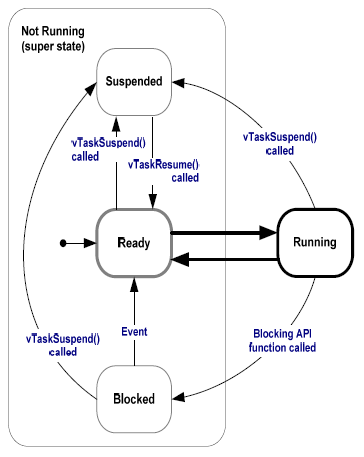
\includegraphics[width=0.3\textwidth]{Pictures/FreeRTOSOrg/taskStates.png}
	\caption{Task States. Quelle~\protect\citeA{MasteringFreeRtos} - Not referenced yet}
	\label{fig:TaskStates}
\end{figure}

Da in FreeRTOS jeder Task eine gewisse Priorität zugewiesen wird, gibt es auch für jede Priorität genau eine Liste, welche alle Tasks dieser Priorität verwaltet. Der FreeRTOS Scheduling Algorithmus kann durch Konfigurations Präprozessor-defines angepasst werden. Der Scheduler kann entweder im Coperative Modus oder im Preemption modus ausgeführt werden. Die Konfiguration wird durch das define configUSE\_PREEMPTION geändert. Im Preemtive Modus wird eine aktive Task mit niedriger Priorität sofort von einer Task mit höherer Priorität verdrängt und ein Kontextwechsel wird durchgeführte. Im kooperativen Modus hingegen wird ein Taskwechsel erst durchgeführt, wenn eine Task den Prozessor explizit abgibt z.B. durch TaskYield(). Abbildung \ref{PreVSCo} zeigt den Vergleich beider Modis durch einen beispielhaften Ablauf. Eine weitere Option die sich über das define configUSE\_TIME\_SLICING aktivieren lässt ist das Time Slicing. Durch Time Slicing wird die zugeteilte Prozessorzeit für Task gleicher Priorität gleichmäßig aufgeteilt. Dies geschieht durch Einführung fester TickInterrupt Intervalle. Bei jedem TickInterrupt überprüft der Scheduler ob sich eine Task gleicher Priorität im Ready Zustand befindet. Sollte es eine solche Task geben wird ein Kontextwechsel durchgeführt und die Task erhält den Prozessor zugeteilt. Die häufigst verwendete Scheduling Algorithmus nennt sich Prioritized Pre-emptive Scheduling with Time Slicing.


\begin{itemize}
	\item Tickcount
	\item FSM
	\item IDLE Task
	\item Priorität nicht durch Scheduler
\end{itemize}
                   
 

Idle Task darf nicht blockiert werden. Idle Task automatisch erstellt nach vTaskStartScheduler. Idle Task räumt auf.  
Blocked - Running :D FSM fertig
Scheduler ändert die Priorität nicht, Änderungen sind aber erlaubt.
Pre-emption : hohe Prio haut low Prio raus
Round Robin : Task dürfen sich abwechseln in dem der Kontext gesichert wird und der Kontext einer anderen Task geladen wird.
Task mit gleicher Prio wechseln sich ab
Time Slicing: verteilt die processing Zeit auf Task mit gleicher Prio, indem nach jedem Zeitschlitz ein Taskwechsel durchgeführt wird.

Cooperative Scheduling in dem Preemption deaktiviert. task wechsel durch task yield.
Leichter externe ressourcen zu managen in Coopoerative, da der task wechsel selbst bestimmt werden kann. 

\begin{figure}[ht!]
	\centering
		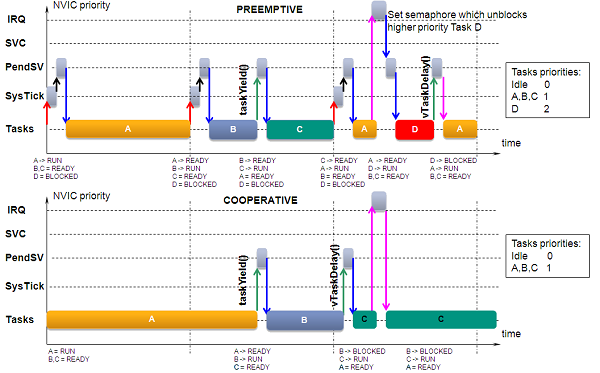
\includegraphics[width=0.5\textwidth]{Pictures/EMCUIT/PreemptiveCooperative.png}
	\caption{Pre-emptive vs. Co-operative. Quelle~\protect\citeA{MasteringFreeRtos} - Not referenced yet}
	\label{fig:PreVSCo}
\end{figure}

\begin{lstlisting}[caption={Implementierung von SysTick aus Task.c}, linewidth=8cm,captionpos=b, label=lst:SysTickS, float=hbt]
void xPortSysTickHandler( void ){
	/* The SysTick runs at the lowest interrupt priority, so when this interrupt
	executes all interrupts must be unmasked.  There is therefore no need to
	save and then restore the interrupt mask value as its value is already
	known. */
	portDISABLE_INTERRUPTS();
	{
		/* Increment the RTOS tick. */
		if( xTaskIncrementTick() != pdFALSE )
		{
			/* A context switch is required.  Context switching is performed in
			the PendSV interrupt.  Pend the PendSV interrupt. */
			portNVIC_INT_CTRL_REG = portNVIC_PENDSVSET_BIT;
		}
	}
	portENABLE_INTERRUPTS();
}
\begin{lstlisting}

\begin{lstlisting}[caption={Pre-emptive List selection aus Task.c}, linewidth=8cm,captionpos=b, label=lst:nextTask, float=hbt]
#define taskSELECT_HIGHEST_PRIORITY_TASK(){																									
	UBaseType_t uxTopPriority = uxTopReadyPriority;														
																										
		/* Find the highest priority queue that contains ready tasks. */								
		while( listLIST_IS_EMPTY( &( pxReadyTasksLists[ uxTopPriority ] ) ) )							
		{																								
			configASSERT( uxTopPriority );																
			--uxTopPriority;																			
		}																								
		/* listGET_OWNER_OF_NEXT_ENTRY indexes through the list, so the tasks of						
		the	same priority get an equal share of the processor time. */									
		listGET_OWNER_OF_NEXT_ENTRY( pxCurrentTCB, &( pxReadyTasksLists[ uxTopPriority ] ) );			
		uxTopReadyPriority = uxTopPriority;																
	} /* taskSELECT_HIGHEST_PRIORITY_TASK */
\end{lstlisting}

\begin{lstlisting}[caption={Implementierung von Kontextwechsel aus Task.c}, linewidth=8cm,captionpos=b, label=lst:taskSwitch, float=hbt]
void vTaskSwitchContext( void )
{
	if( uxSchedulerSuspended != ( UBaseType_t ) pdFALSE )
	{
		/* The scheduler is currently suspended - do not allow a context
		switch. */
		xYieldPending = pdTRUE;
	}
	else
	{
		xYieldPending = pdFALSE;
		/* Check for stack overflow, if configured. */
		taskCHECK_FOR_STACK_OVERFLOW();
		/* Select a new task to run using either the generic C or port
		optimised asm code. */
		taskSELECT_HIGHEST_PRIORITY_TASK();
		traceTASK_SWITCHED_IN();
	}
}
\end{lstlisting}



\begin{figure}[ht!]
	\centering
		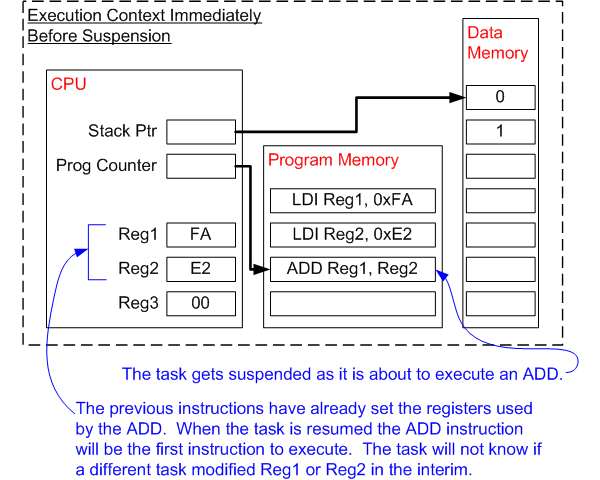
\includegraphics[width=0.4\textwidth]{Pictures/FreeRTOSOrg/ExeContext.png}
	\caption{FreeRTOS Pseudoimplementierung des Context - Switch. Quelle~\protect\citeA{MasteringFreeRtos} - Not referenced yet}
	\label{fig:FreeRTOSFsm}
	
\end{figure}

\begin{figure}[ht!]
	\centering
		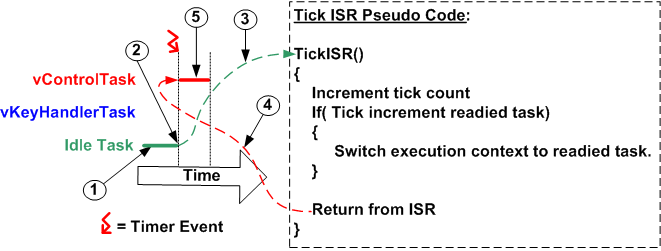
\includegraphics[width=0.4\textwidth]{Pictures/FreeRTOSOrg/TickISR.png}
	\caption{FreeRTOS Pseudoimplementierung des Tick Interrupts. Quelle~\protect\citeA{MasteringFreeRtos} - Not referenced yet}
	\label{fig:FreeRTOSFsm}
\end{figure}